\begin{figure}[htb!]
\centering
\begin{tabular}{ccc}
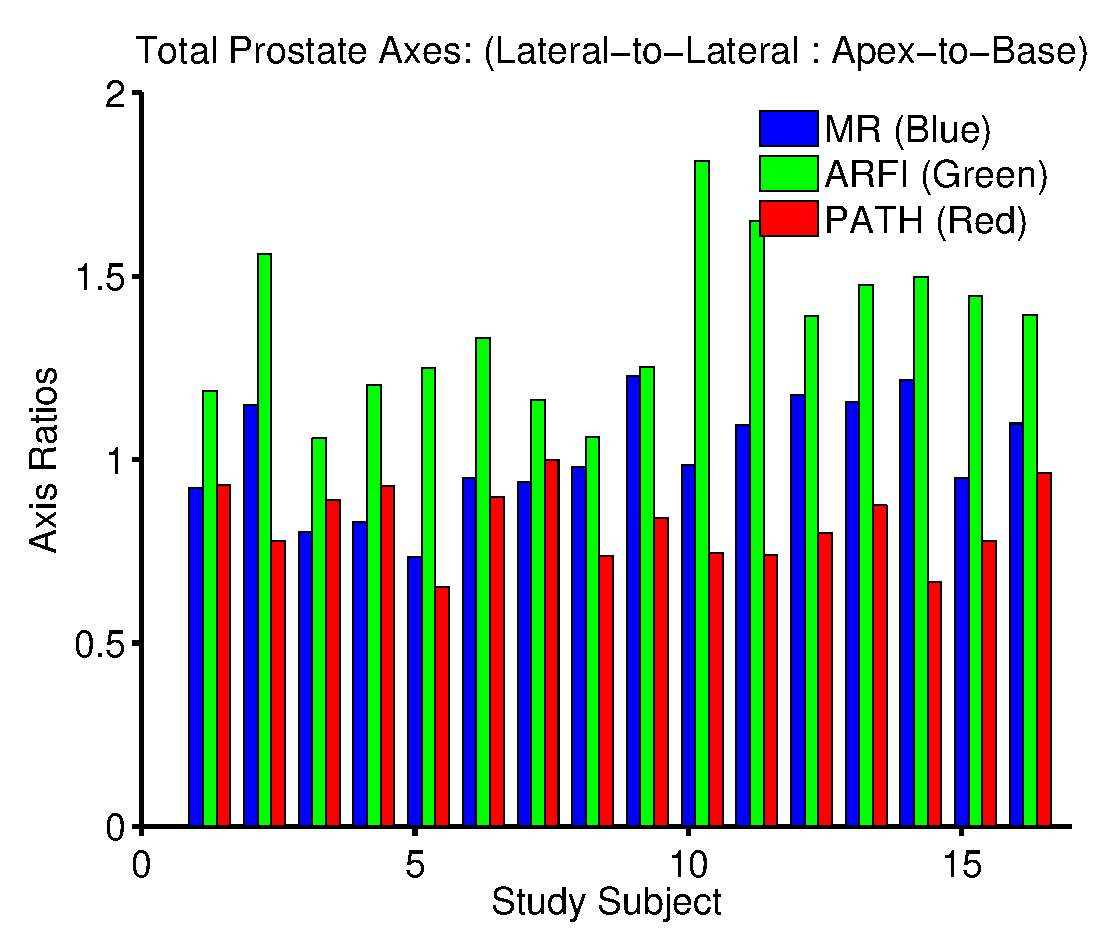
\includegraphics[width=0.3\linewidth]{figs/mr_arfi_total_axes1} &
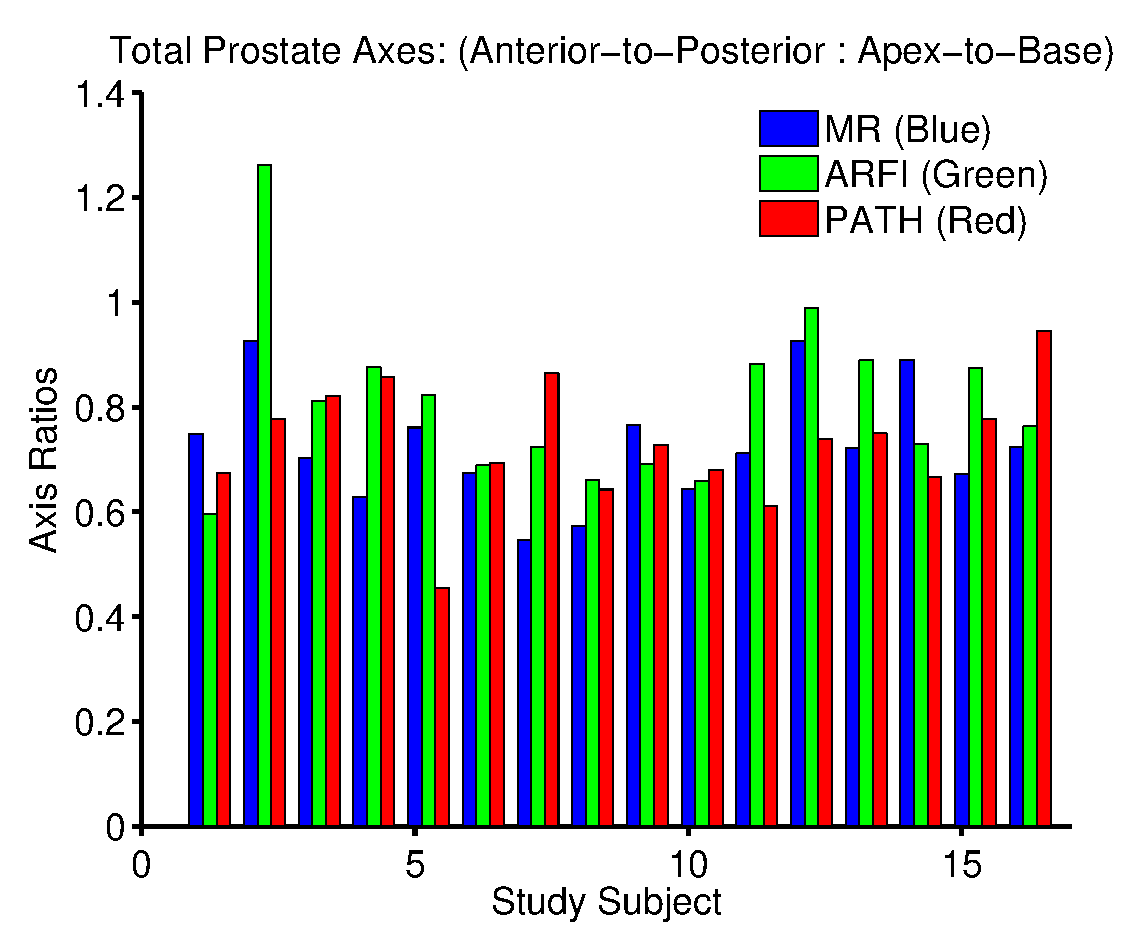
\includegraphics[width=0.3\linewidth]{figs/mr_arfi_total_axes2} &
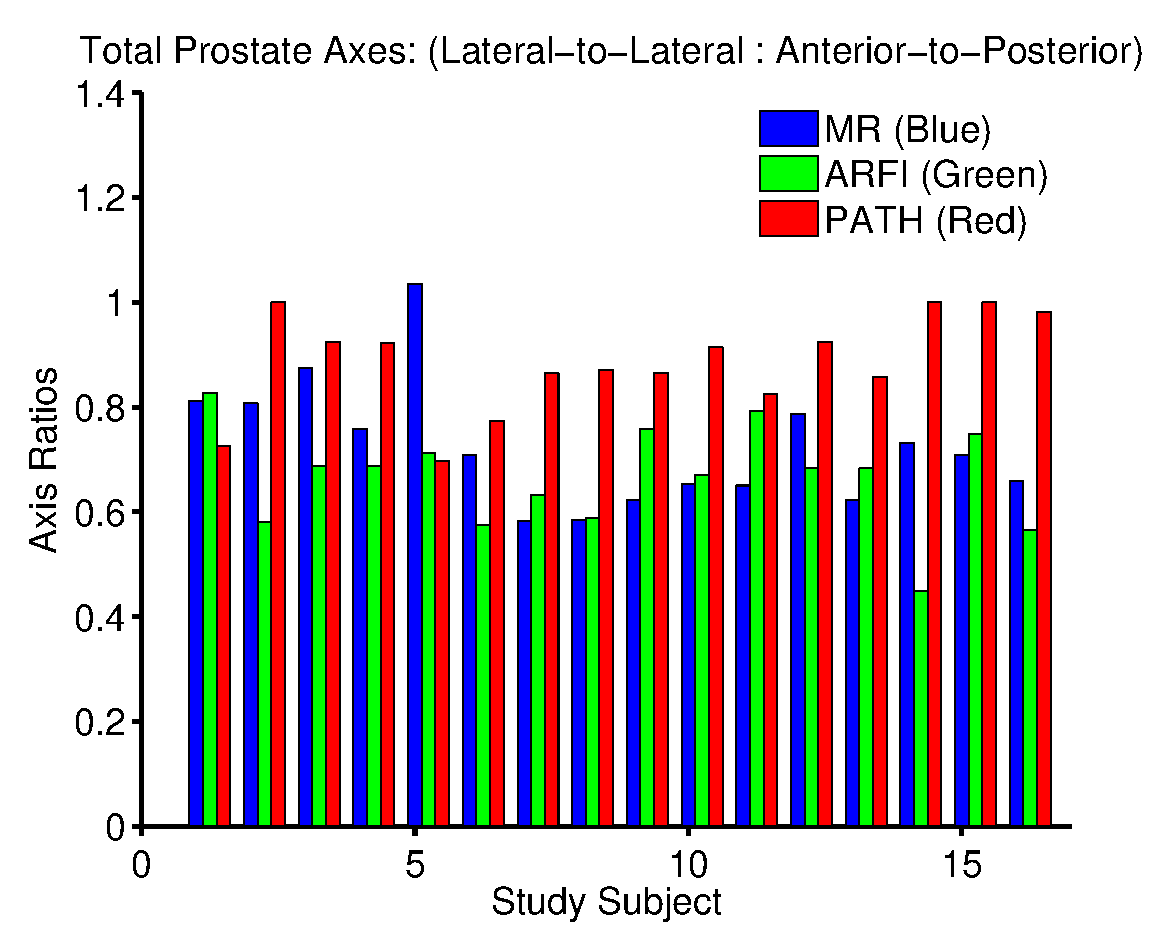
\includegraphics[width=0.3\linewidth]{figs/mr_arfi_total_axes3} \\
(a) & (b) & (c) \\
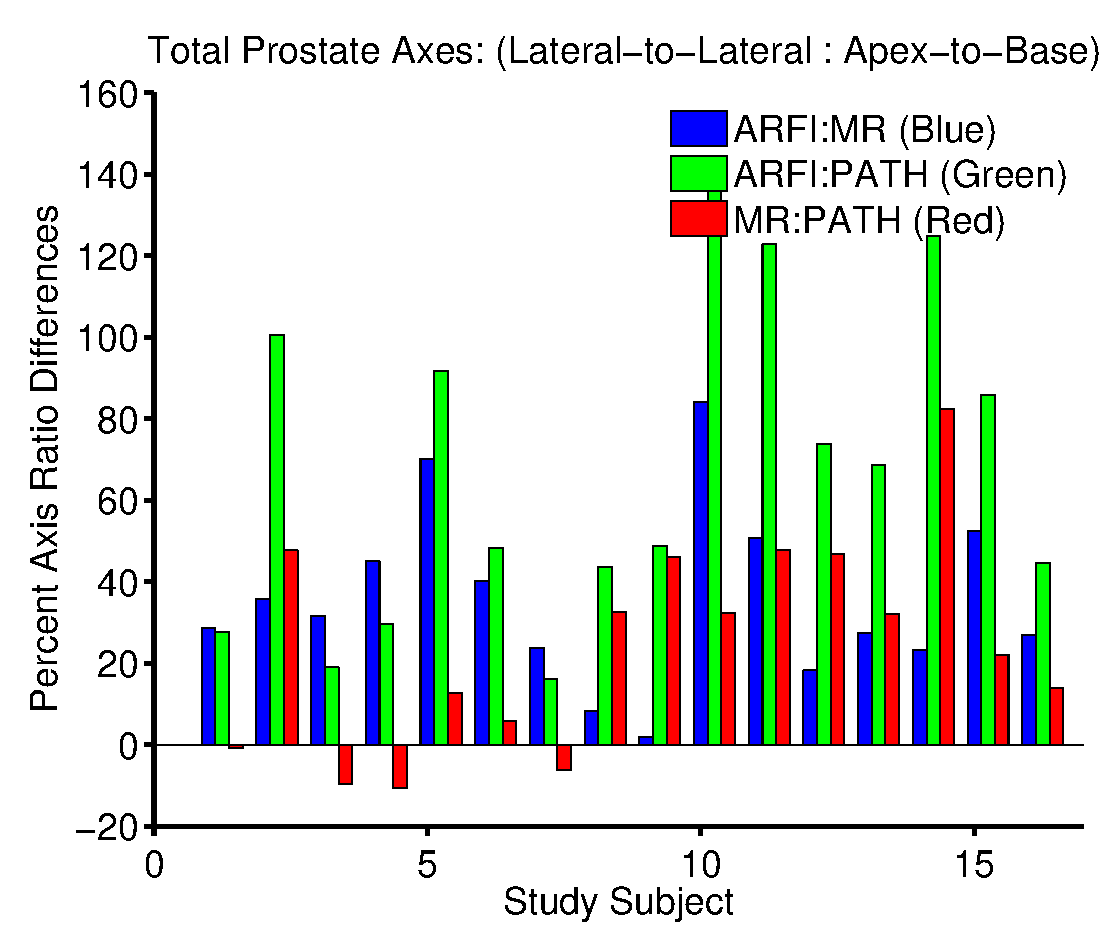
\includegraphics[width=0.3\linewidth]{figs/mr_arfi_total_over_under1} &
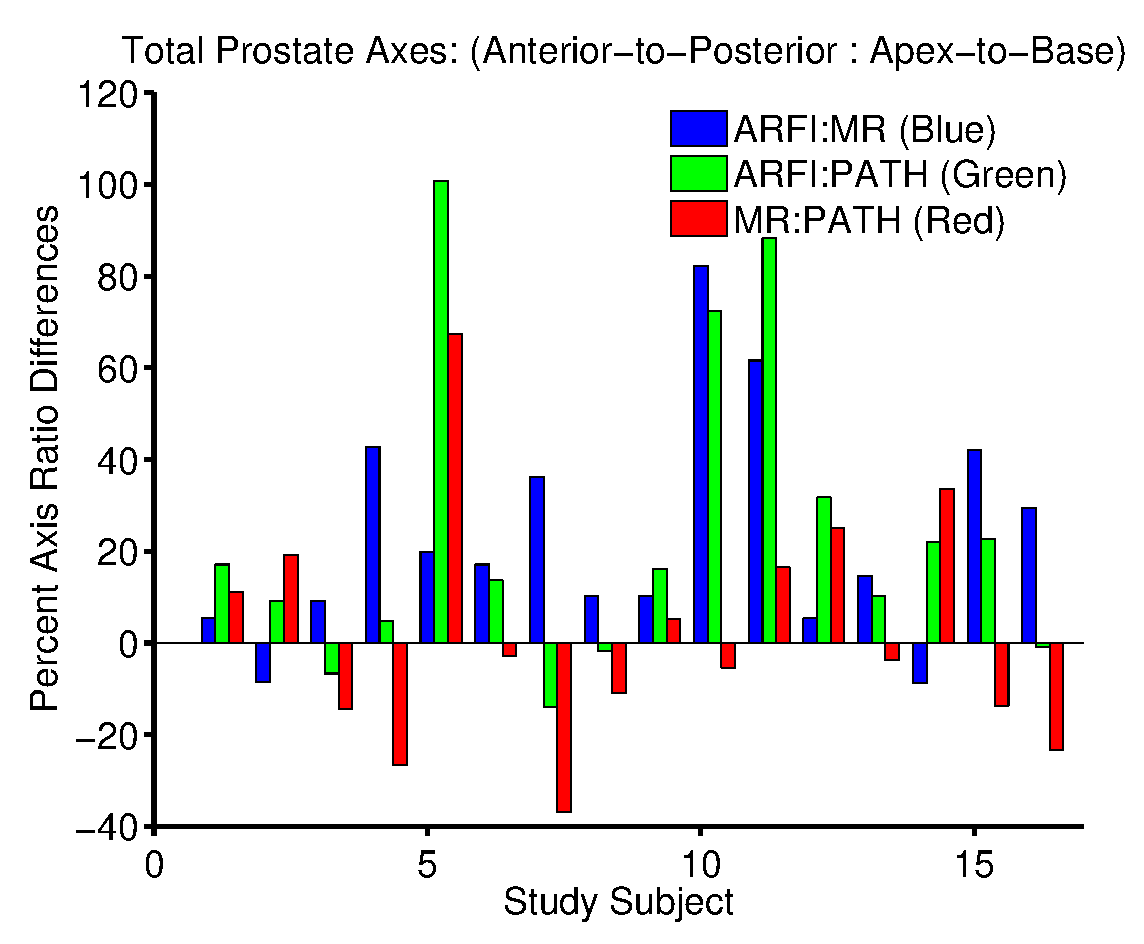
\includegraphics[width=0.3\linewidth]{figs/mr_arfi_total_over_under2} &
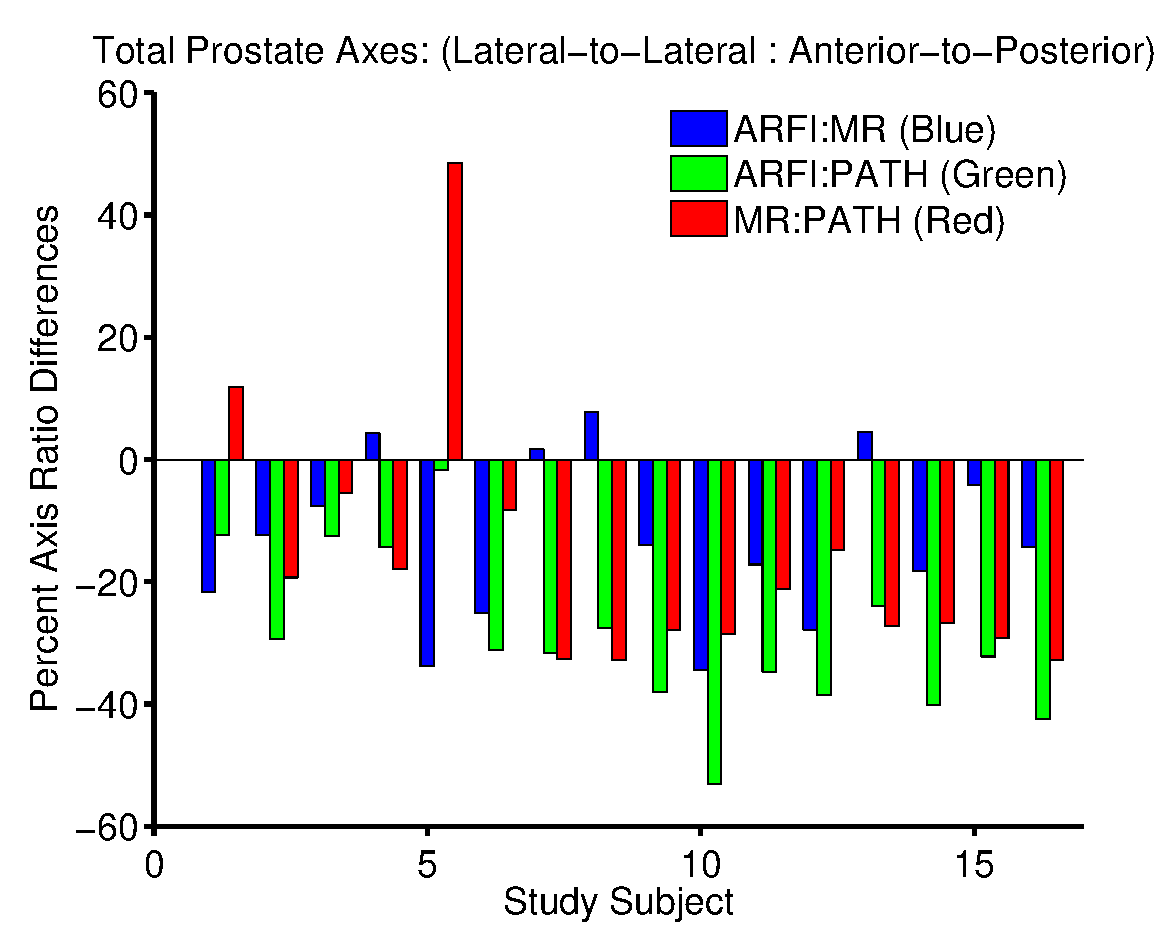
\includegraphics[width=0.3\linewidth]{figs/mr_arfi_total_over_under3} \\
(d) & (e) & (f) \\
\end{tabular}
\caption{Comparison of the ratios of the three anatomic axis measurement ratios
    for T2WI MR (top row, blue), ARFI imaging (top row, green) and gross
    pathology (top row, red).  The over/underestimation of the axis ratios
    between ARFI imaging : T2WI MR : Pathology are shown in the bottom row
    (d-f), with mean ratio differences compiled in
    Table~\ref{tab:axis_ratio_over_under}.}
\label{fig:mr_arfi_total_axes} 
\end{figure}
